\documentclass[../../main.tex]{subfiles}
\begin{document}

\subsection*{8.10}
Due conduttori cilindrici molto lunghi di raggio R, paralleli tra loro a notevole distanza l'uno dall'altro, sono percorsi dalle correnti $i_1$ e $i_2$ in versi opposti.\\
La circuitazione del campo magnetico lungo i percorsi chiusi $C_1$ e $C_2$ indicati in figura vale rispettivamente $\Gamma_1(B) = 0$ e $\Gamma_2(B) = -20\pi * 10^{-7}\ Tm$.\\
Calcolare $i_1$ e $i_2$.\\
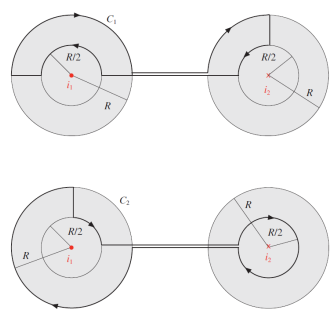
\includegraphics[scale=0.3]{e_8_10.png}
\subsubsection*{Formule utilizzate}
\subsubsection*{Soluzione punto a}
\subsubsection*{Soluzione punto b}
\newpage

\end{document}